\section{Metodologia e Resultados}

\subsection{Coleta de Dados}

Os dados utilizados neste trabalho foram obtidos de dados históricos de opções sobre o ativo $SPY$, da bolsa estadunidense, de 2021 à 2022, disponível no \href{https://www.kaggle.com/datasets/shawlu/option-spy-dataset-combinedcsv}{Kaggle}. Este conjunto de dados contém diversas colunas sobre opções negociadas, indexadas pela data, incluindo preços de exercício, preços futuros, maturidades, volatilidades implícitas, entre outros \citep{}. O arquivo pode ser e foi baixado e armazenado localmente em um diretório específico para processamento.

\subsection{Descrição do Conjunto de Dados}

O conjunto de dados contém as seguintes colunas relevantes para nosso estudo, além de diversas outras:
\begin{itemize}
	\item \textbf{underlying}: Preço do ativo subjacente.
	\item \textbf{strike}: Preço de exercício da opção.
	\item \textbf{daysToExpiration}: Dias restantes até a expiração da opção.
	\item \textbf{iv}: Volatilidade implícita.
	\item \textbf{dt}: Data do registro.
\end{itemize}

Além disso, adicionamos duas colunas calculadas:
\begin{itemize}
	\item \textbf{maturity}: Calculada dividindo \textit{daysToExpiration} por 360 (dias úteis no ano) para normalizar o tempo de maturidade.
	\item \textbf{r}: Taxa livre de risco obtida do Federal Reserve Economic Data (FRED) para o período correspondente.
	\item \textbf{d}: Taxa de dividendos paga trimestralmente pelo SPY.
\end{itemize}

\subsection{Pré-processamento dos Dados}

O pré-processamento dos dados encorreu em várias etapas essenciais, predominantemente realizadas para permitir o uso dos dados diretamente na arquitetura do transformer e subsequente uso para gerar a superfície para os dados históricos. O transformer tem como entrada 4 dimensões, sendo elas: 
\begin{enumerate}
\item O tempo até a maturidade; 
\item O valor do parâmetro ($\alpha, \rho$, ou $\nu$); 
\item $\mathbf{1}$ se o parâmetro foi calculado para o dia atual, $\mathbf{0}$ se foi calculado no dia anterior por não existir no dia atual; 
\item Parâmetros calculados utilizando as pontuações do dia anterior.
\end{enumerate}

A variável target são os scores gerados utilizando-se todos os pontos candidatos para o dia atual, e a função de erro do modelo utiliza uma porcentagem \textbf{p} de pontos e é treinado para minimizar a função de erro quadrática das pontuações.

\subsection{Métricas de Erro e Comparação das Superfícies}

Utilizamos como baseline uma interpolação linear dos pontos observados diariamente, e comparamos com a performance do modelo em relação à pontos internos à uma malha (ou \textit{grid} em inglês) gerada para pontos dentro do intervalo diário, tanto para valores de maturidade como de \textit{strike}.

O nosso modelo transformer foi treinado em cima do conjunto de dados, de aproximadamente 70 observações, cada uma com uma sequência de em média 700 pontos. Os modelos foram treinados por aproximadamente 700 épocas.

\begin{figure}
	\begin{center}
		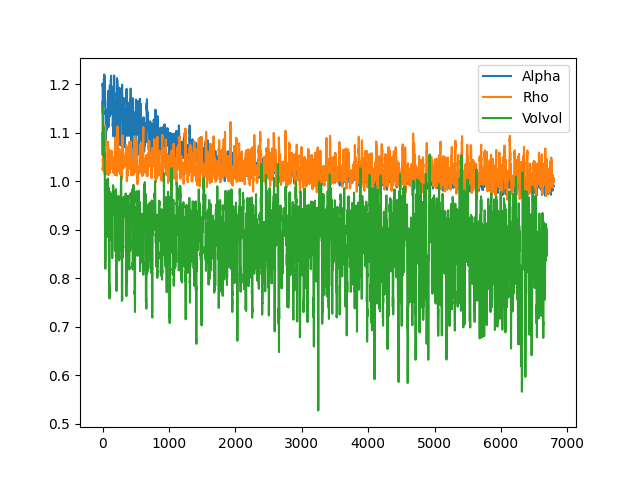
\includegraphics[width=8cm]{resources/losses.png}
		\caption{Função de perda histórica, de uma sessão de treinamento do Transformer}
	\end{center}
\end{figure}
	
\begin{figure}
	\begin{center}
		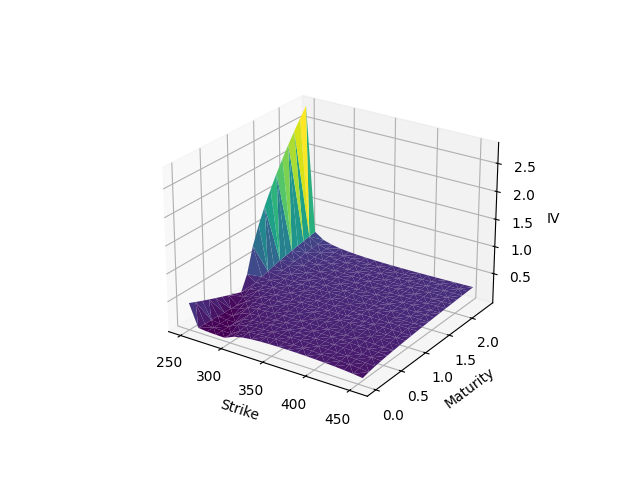
\includegraphics[width=8cm]{resources/pred_surface.png}
		\caption{Superfície gerada utilizando um modelo SABR com parâmetros otimizados manualmente. Note que a não-remoção de \textit{outliers} gerou um pico na superfície}
	\end{center}
\end{figure}

\begin{figure}
	\begin{center}
		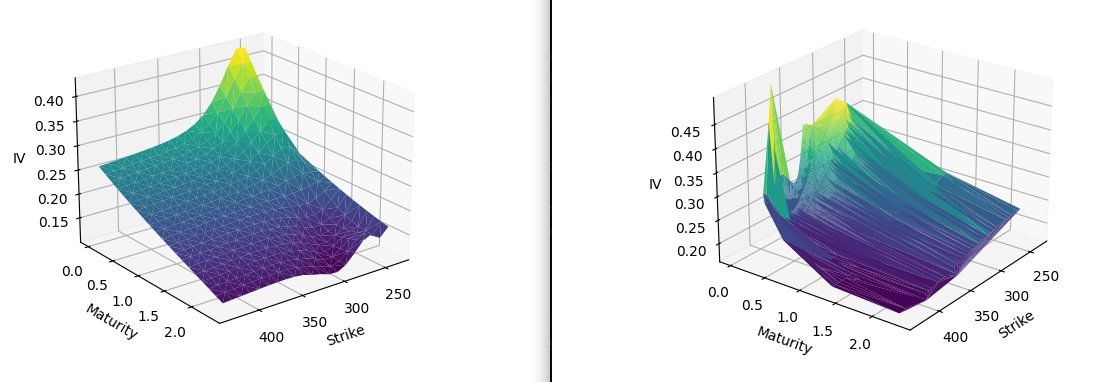
\includegraphics[width=16cm]{resources/sst.png}
		\caption{Comparação da superfície real com a gerada após treinamento do Transformer. Na esquerda, a superfície do modelo SST, na direita, a superfície interpolada linearmente}
	\end{center}
\end{figure}
	
